\documentclass{beamer}

\usepackage{amsmath,amssymb,amsfonts}
\usepackage{graphicx}
\usepackage[round]{natbib}
\usepackage{booktabs}
\usepackage{hyperref}
\usepackage{setspace}
\usepackage{lmodern} % for better font rendering
\usepackage{caption} % for table captions
\usepackage{adjustbox} % to resize tables if needed
\usepackage{multirow}

\usetheme{Madrid}
\usecolortheme{default}

% For references in footnotesize
\setbeamertemplate{bibliography item}[text]

\title[Generative AI and Labor Demand]{Generative AI and Labor Demand:\\
Evidence from Online Job Markets}
\author[Georgi Demirev]{Georgi Demirev\\
\footnotesize Sofia University St. Kliment Ohridski\\
Ryan Institute on Complexity, Northwestern University (visiting)}
\date{\today}

\begin{document}
% -------------------------------------------------------------------
\begin{frame}
  \titlepage
\end{frame}

% -------------------------------------------------------------------
\begin{frame}{Outline}
  \tableofcontents
\end{frame}

% -------------------------------------------------------------------
\section{Introduction and Motivation}
\begin{frame}{Motivation}
\begin{itemize}
    \item The empirical record on AI and employment is surprisingly mixed:
    \begin{itemize}
        \item Firm surveys: widespread adoption, modest employment effects \citep{yotzov2026firmdata}
        \item Administrative data: precise null on earnings and hours \citep{humlum2025stillwaters}
        \item Freelance platforms: meaningful contractions for writing- and coding-intensive tasks \citep{demirci2025replacing, hui2023shortterm}
    \end{itemize}
    \item Much of the difficulty stems from the granularity and timeliness of available data, especially outside the US.
    \item This paper: high-frequency online job postings across the EU (CEDEFOP Skills OVATE), five task-based AI exposure measures, ChatGPT release as the event date.
\end{itemize}
\end{frame}

\begin{frame}{Research Question and Contributions}
    \textbf{Are occupations with higher exposure to AI experiencing worse labor demand outcomes relative to occupations with lower exposure?}

    \vspace{0.4cm}
    Relative to the existing empirical literature:
    \begin{itemize}
        \item European evidence to complement the largely US-focused work
        \item Within-occupation skill-level analysis, not only across occupations
        \item Heterogeneity by experience level
        \item Out-of-sample validation on Australian data
    \end{itemize}
\end{frame}

\begin{frame}{Key Findings}
\begin{itemize}
    \item Occupations at the highest levels of AI exposure see a \textbf{19--29\% relative decrease} in EU job postings since the release of ChatGPT, robust across five exposure measures.
    \item Partially replicated out-of-sample on Australian data (the two most recent measures).
    \item Within occupations, skills most similar to AI capabilities are mentioned \textbf{12\% less frequently}.
    \item \textbf{No significant impact} on industry-level labor or capital productivity, consistent with ``so-so automation''.
    \item Inverted U-shape in experience: the decline concentrates in entry-level postings and those requiring 10+ years of experience.
\end{itemize}
\end{frame}

% -------------------------------------------------------------------
\section{Conceptual Framework}
\begin{frame}{Task-Based Framework}
\begin{itemize}
    \item Task-based model of automation \citep{zeira1998workers, acemoglu_restrepo_2022}: sector output is an aggregate of task outputs, each produced by labor or AI.
    \item Sector exposure = share of the labor force employed in tasks about to be automated:
\end{itemize}
\begin{equation*}
d\ln{l_s} = (-1 + (\epsilon_s\rho_s-1)\pi_s)\times exposureAI_s
\end{equation*}
\begin{itemize}
    \item The sign is theoretically ambiguous:
    \begin{itemize}
        \item Displacement dominates $\Rightarrow$ employment falls with exposure
        \item Large enough productivity gains (elastic demand, high pass-through) $\Rightarrow$ employment can expand
    \end{itemize}
    \item Which effect dominates is an empirical question for any given technology.
\end{itemize}
\end{frame}

% -------------------------------------------------------------------
\section{Data}
\begin{frame}{Five Measures of Occupational AI Exposure}
\footnotesize
\begin{table}
\begin{tabular}{lll}
\toprule
Measure & Source data & Vintage \\
\midrule
\citet{felten_method_2018} & Crowd-sourced ability--application links & pre-LLM \\
\citet{webb_impact_2022} & AI patents matched to O*NET tasks & pre-LLM \\
\citet{eloundou_gpts_2023} & GPT-4 rates its own automation potential & post-LLM \\
\citet{demirev2024assessing} & AI product press releases vs.\ ESCO skills & post-LLM \\
\citet{handa2025economic} & Observed Claude.ai usage by O*NET task & post-LLM \\
\bottomrule
\end{tabular}
\end{table}
\normalsize
\begin{itemize}
    \item All rescaled to $[0,1]$; results reported separately for each measure.
    \item \citet{demirev2024assessing} and \citet{handa2025economic} additionally split exposure into ``automation'' vs.\ ``augmentation''.
    \item \citet{demirev2024assessing} also provides skill-level exposure, used for the within-occupation analysis.
\end{itemize}
\end{frame}

\begin{frame}{Job Postings and Productivity Data}
\begin{itemize}
    \item \textbf{Skills OVATE (CEDEFOP/Eurostat):} 100M+ online job adverts across the EU, Q4 2021--Q2 2025; occupations (ESCO level 3) and skill mentions by country.
    \item \textbf{EURES:} vacancies by required experience level; only available from Q3 2024, so used descriptively.
    \item \textbf{Australian Internet Vacancy Index:} ANZSCO 4-digit vacancies by state, 2016--2026; a full decade of pre-trends.
    \item \textbf{Eurostat national accounts (nama10):} labor and capital productivity by NACE industry, 2021--2024.
    \item Caveat: online job openings are only a proxy of real labor demand (``ghost listings'', uneven coverage across occupations).
\end{itemize}
\end{frame}

\begin{frame}{The Overall Market Contracted Sharply}
\begin{figure}
    \centering
    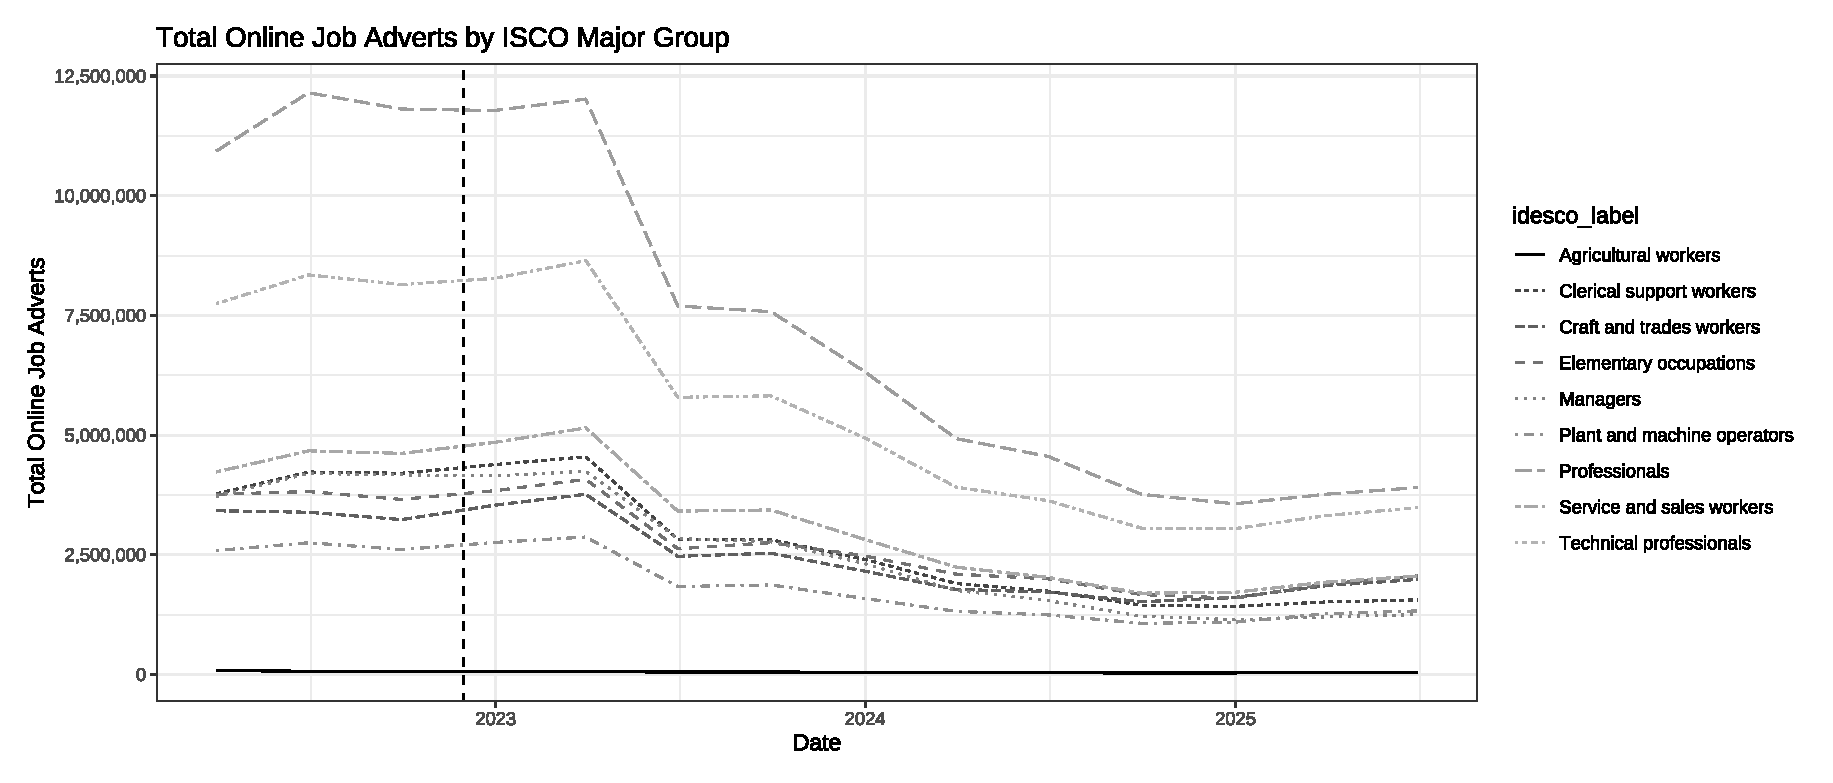
\includegraphics[width=0.62\textwidth]{img/oja_time_series.eps}
    \caption{\small Total online job adverts by ESCO level-1 occupation (rolling 12-month totals). Source: \citet{cedefop_skills_ovate}}
\end{figure}
\vspace{-0.3cm}
\footnotesize From 40.3M adverts (early 2022) to 17.7M (mid 2025), a 50\%+ decline, steeper than any comparable benchmark. All specifications compare occupations \emph{within} each period.
\end{frame}

% -------------------------------------------------------------------
\section{Empirical Strategy}
\begin{frame}{Long-Difference Specification}
Difference-in-differences with continuous treatment; event date is the release of ChatGPT (November 2022):
\begin{equation*}
    \Delta\log{\bar{y}}_{c,i} = \delta_0 + \xi_c + \delta X^{AI}_i + \varepsilon_{c,i}
\end{equation*}
\begin{itemize}
    \item $\Delta\log{\bar{y}}_{c,i}$: change in log average job postings per quarter, pre vs.\ post event, for occupation $i$ in country $c$
    \item $X^{AI}_i$: one of the five exposure measures, scaled to $[0,1]$
    \item $\xi_c$: country fixed effects; standard errors clustered by country
    \item Event-study version with country-occupation fixed effects tests for pre-trends
    \item Analogous specifications for skills (occupation FE added), experience levels, and industry productivity
\end{itemize}
\end{frame}

% -------------------------------------------------------------------
\section{Results}
\begin{frame}{Main Result: AI Exposure and Job Postings}
\begin{table}
\centering
\scriptsize
\caption{Impact of AI Exposure on Online Job Ads ($\Delta \log(\text{OJA})$)}
\begin{tabular}{lccccc}
\toprule
 & (1) & (2) & (3) & (4) & (5) \\
\midrule
Demirev Exposure & -0.211*** & & & & \\
 & (0.055) & & & & \\
Felten AI Exposure & & -0.212** & & & \\
 & & (0.058) & & & \\
Webb AI Exposure & & & -0.205*** & & \\
 & & & (0.043) & & \\
Eloundou Exposure & & & & -0.289*** & \\
 & & & & (0.066) & \\
Anthropic Usage & & & & & -0.339*** \\
 & & & & & (0.054) \\
\midrule
Observations & 2,788 & 2,785 & 2,776 & 2,785 & 2,785 \\
R$^2$ (within) & 0.013 & 0.026 & 0.016 & 0.034 & 0.017 \\
Country FE & Yes & Yes & Yes & Yes & Yes \\
\bottomrule
\multicolumn{6}{l}{\tiny Standard errors clustered at country level. * p$<$0.05, ** p$<$0.01, *** p$<$0.001} \\
\end{tabular}
\end{table}
\footnotesize Moving from lowest to highest exposure: \textbf{19--29\% relative decrease} in postings. Significant for all five measures.
\end{frame}

\begin{frame}{Visual Illustration: Partial Correlation}
\begin{figure}
    \centering
    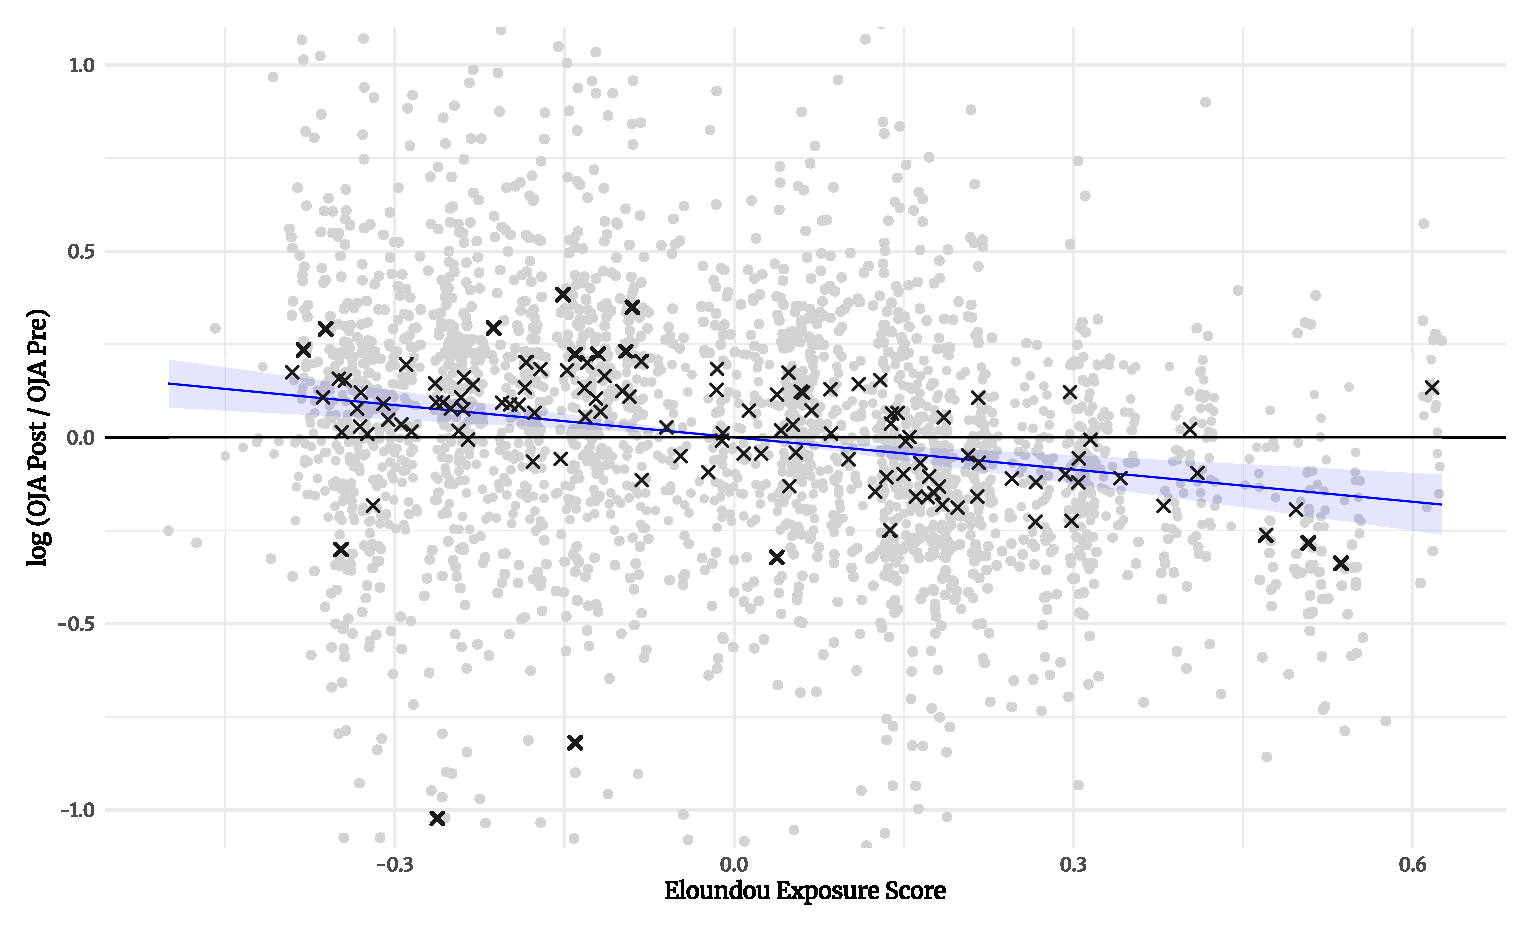
\includegraphics[width=0.62\textwidth]{img/partial_plots_eloundou.eps}
    \caption{\small Partial correlation of AI exposure and $\Delta \log(\text{OJA})$, residualized on country FE (Eloundou measure). Dots: country-occupation pairs; crosses: occupation averages.}
\end{figure}
\vspace{-0.3cm}
\footnotesize Within-country R$^2$ is small (0.013--0.034): AI exposure explains little of the overall contraction, but predicts \emph{where} it concentrates.
\end{frame}

\begin{frame}{Event Study: The Effect Grows Over Time}
\begin{figure}
    \centering
    
\includegraphics[width=0.68\textwidth]{img/event_study_all.eps}
    \caption{\small Event-study coefficients around the ChatGPT release, all five measures.}
\end{figure}
\vspace{-0.3cm}
\footnotesize Significant negative coefficients from 2 quarters post-event, growing to 46--59\% by mid-2025 (Webb is the exception). Some significant pre-event coefficients; addressed with the longer Australian pre-period.
\end{frame}

\begin{frame}{Automation vs.\ Augmentation}
\begin{table}
\centering
\small
\caption{Impact on OJA by Intent ($\Delta \log(\text{OJA})$)}
\begin{tabular}{lcc}
\toprule
 & Handa & Demirev \\
\midrule
Automation Exposure & -0.236** & 0.064 \\
 & (0.064) & (0.050) \\
Augmentation Exposure & 0.137* & -0.277*** \\
 & (0.059) & (0.069) \\
\midrule
Observations & 2,785 & 2,788 \\
Country FE & Yes & Yes \\
\bottomrule
\multicolumn{3}{l}{\tiny Clustered (by country) SEs. * p$<$0.05, ** p$<$0.01, *** p$<$0.001} \\
\end{tabular}
\end{table}
\begin{itemize}
    \item \citet{handa2025economic}: demand falls for automatable jobs, rises where AI augments workers.
    \item \citet{demirev2024assessing} does not separate as cleanly; its intent breakdown should be treated as suggestive.
\end{itemize}
\end{frame}

\begin{frame}{Out-of-Sample Validation: Australia}
\begin{figure}
    \centering
    
\includegraphics[width=0.49\textwidth]{img/aus_event_study_l3_demirev.eps}
    
\includegraphics[width=0.49\textwidth]{img/aus_event_study_l3_anthropic.eps}
\end{figure}
\vspace{-0.2cm}
\footnotesize
\begin{itemize}
    \item The two most recent measures replicate: Anthropic Usage $-0.357$ (0.036), Demirev $-0.152$ (0.025), i.e.\ 14--30\% relative reduction.
    \item Felten is significant but \emph{positive}; Webb and Eloundou insignificant.
    \item A decade of pre-trends, reaching through COVID (shaded): no evidence the post-ChatGPT decline is reversion-to-the-mean.
\end{itemize}
\end{frame}

\begin{frame}{Skill-Level Demand Within Occupations}
\begin{columns}
\begin{column}{0.48\textwidth}
\begin{table}
\centering
\scriptsize
\begin{tabular}{lc}
\toprule
Dep.\ var.: & $\Delta \log(\text{Skill Mentions})$ \\
\midrule
AI Product Exposure & -0.246* \\
 & (0.113) \\
\midrule
Observations & 75,669 \\
Occupation FE & Yes \\
Country FE & Yes \\
\bottomrule
\multicolumn{2}{l}{\tiny SEs clustered by country and occupation.} \\
\end{tabular}
\end{table}
\end{column}
\begin{column}{0.5\textwidth}
\footnotesize
\begin{itemize}
    \item Most exposed skill in the sample: roughly \textbf{12\% fewer mentions} post-GPT, net of occupational composition (occupation FE).
    \item Suggests changes in task composition within occupations.
    \item Caveat: significant pre-event coefficients in the event study, so the causal interpretation is weaker here.
\end{itemize}
\end{column}
\end{columns}
\end{frame}

\begin{frame}{Experience Heterogeneity: An Inverted U-Shape}
\begin{figure}
    \centering
    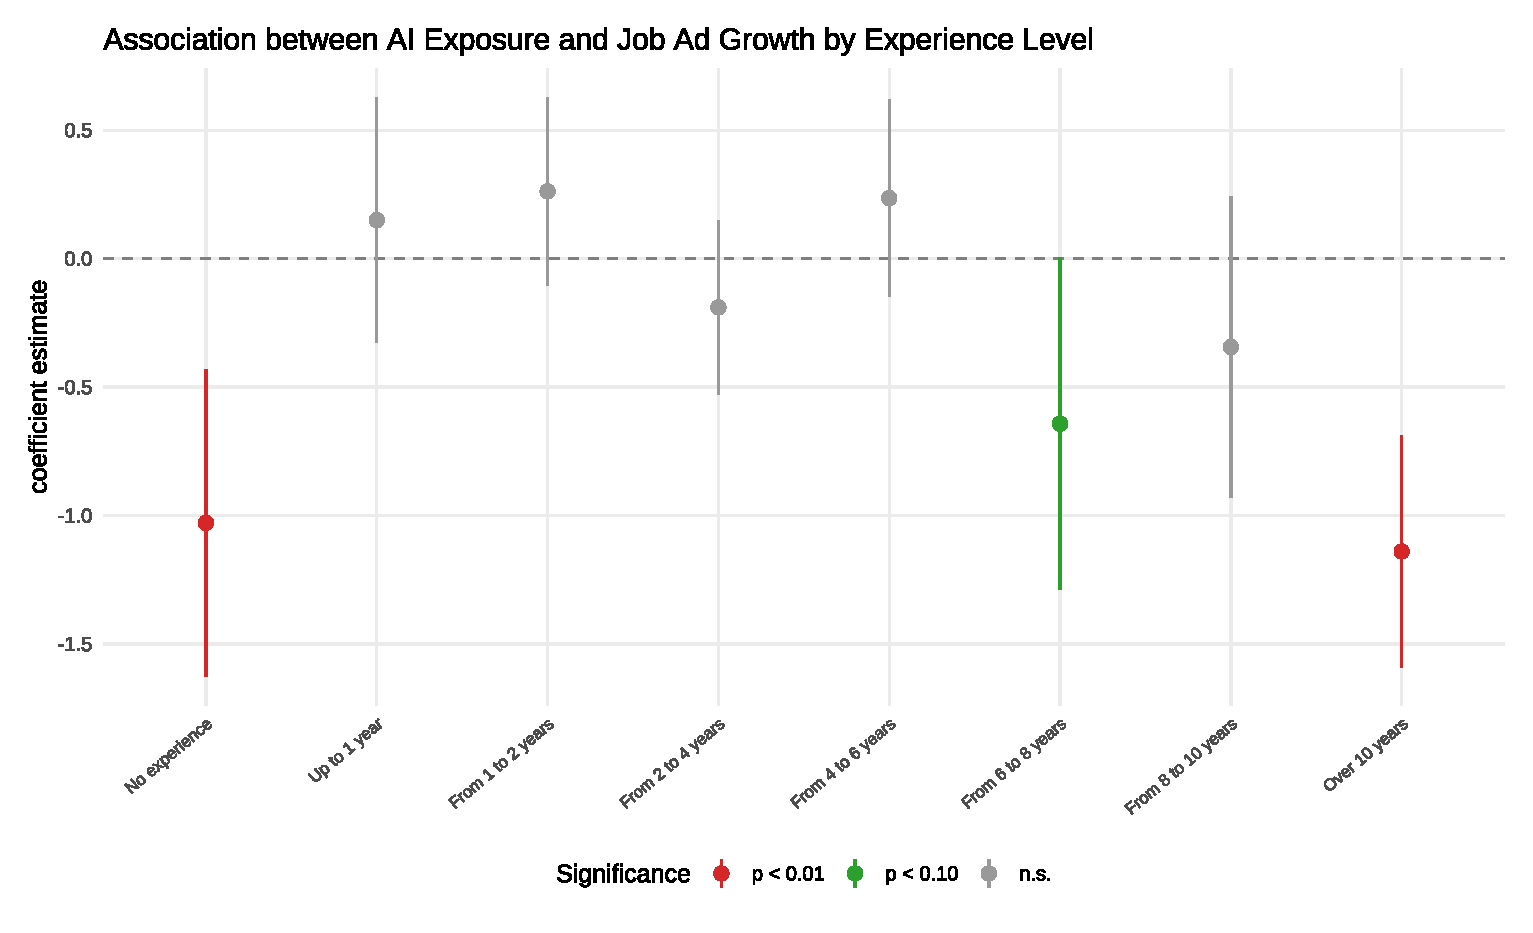
\includegraphics[width=0.66\textwidth]{img/by_experience_anthropic.eps}
    \caption{\small Exposure gradients by experience bin, \citet{handa2025economic} measure (EURES data, 2024Q3--2025Q2, descriptive).}
\end{figure}
\vspace{-0.3cm}
\footnotesize Largest declines at both tails: entry-level \emph{and} 10+ years of experience (36--67\% fewer vacancies at highest exposure). Entry-level echoes \citet{brynjolfsson2025canaries}; the senior tail is new.
\end{frame}

\begin{frame}{Productivity: A Null Result}
\begin{itemize}
    \item Industry exposure scores built from the occupational mix within each industry (ESCO employment weights).
    \item TWFE and long-difference models of labor and capital productivity (Eurostat, 2021--2024).
    \item \textbf{None of the estimated coefficients is significant} for any of the five measures.
    \item The null is informative: displacement appears to operate without a measurable productivity offset at sector-level granularity.
    \item Caveats: annual frequency, series ends six months before the OJA data, only 17 industries.
\end{itemize}
\end{frame}

\begin{frame}{Robustness}
\begin{itemize}
    \item \textbf{Leave-one-out:} dropping any single occupation (level 2 or 3) or country never flips the sign or loses significance, for any measure.
    \item \textbf{TWFE in levels:} all five interaction coefficients negative and significant ($-0.168$ to $-0.483$).
    \item \textbf{Deciles:} broadly monotone; declines concentrated in the top exposure deciles.
    \item \textbf{Teleworkability confound:} the two measures \emph{least} correlated with \citet{dingel2020teleworkable} teleworkability (Demirev, Handa) are exactly the ones that replicate on Australian data, arguing against a remote-work reversion story.
\end{itemize}
\end{frame}

% -------------------------------------------------------------------
\section{Conclusion}
\begin{frame}{Conclusion: ``So-So Automation''?}
\begin{itemize}
    \item Highly exposed occupations show a \textbf{19--29\% relative decline} in job postings post-ChatGPT, growing over time, robust across five exposure measures, and partially replicated in Australia.
    \item Within occupations, AI-similar skills are mentioned up to 12\% less.
    \item No measurable industry-level productivity effect.
    \item Together, consistent with \citet{acemoglu_automation_2019}'s ``so-so automation'': AI does enough to displace parts of labor, but the efficiency gains are insufficient to offset the disemployment effects.
    \item Initial effects only; monitoring labor market outcomes for exposed occupations should remain a priority.
\end{itemize}
\end{frame}

\begin{frame}{Caveats and Limitations}
\begin{itemize}
    \item AI exposure explains little of the \emph{overall} market contraction; it predicts its distribution across occupations.
    \item The post-ChatGPT period coincides with monetary tightening and the unwinding of pandemic-era policies; interest-rate-sensitive sectors (e.g.\ software) rank high on every exposure measure.
    \item Some significant pre-event coefficients in the EU event studies; alleviated but not eliminated by the Australian pre-period and the teleworkability analysis.
    \item Online job adverts are a partial view of the labor market: postings may decline even if employment stays fixed.
\end{itemize}
\end{frame}

% -------------------------------------------------------------------
\section{References}
\begin{frame}[allowframebreaks]{References}
\tiny
\bibliographystyle{plainnat}
\bibliography{references}
\end{frame}

\end{document}
